%%Template made by Uday Khankhoje for examinations using the exam template
%%Refer to the documentation http://www-math.mit.edu/~psh/exam/examdoc.pdf 
%%for lot more bells and whistles to the standard template shown belowva
\documentclass[a4paper,11pt,addpoints]{exam}
\usepackage[left=1.5cm,right=1.5cm,top=1.5cm,bottom=2cm]{geometry}
%\usepackage{mathrsfs}
\usepackage{graphicx,color}
\usepackage[x11names]{xcolor}
\usepackage{venndiagram}
\usepackage{epic,eepic}
%\usepackage{mathpazo}
\usepackage{url}
\usepackage{tasks} % cria lista curta
\usepackage{multicol}
\usepackage{amsmath, amsthm, amssymb}
\pointsinmargin
\boxedpoints 
\renewcommand*\half{.5}
\usepackage{setspace}
\DeclareMathOperator{\vecc}{vec}
%\renewcommand{\vec}[1]{\ensuremath{\mathbf{#1}}}

\global\vbadness=1616

\begin{document}
\noindent 
%%PART 1 of header
\begin{center}
	\vspace*{-3em}
\def\arraystretch{2.0}
\begin{tabular}{|p{0.7\linewidth}|p{0.2\linewidth}|}
\hline 
\textbf{@tema@} & Pontos Obtidos $\downarrow$ \\
\hline 
Data:\hspace{3cm}  Total de questões \textbf{\numquestions} \hspace{1cm} Total de pontos: \textbf{\numpoints} &   \\ 
\hline 
\multicolumn{2}{|l|}{Tuma: \hspace{0.3\linewidth} Nome: \hspace{0.3\linewidth} Duração: 2 hrs} \\
\hline
\end{tabular} 
\end{center}
%%PART 2 of header, if you have too many questions, this may be a problem
%%if so, use \multirowgradetable{n}[questions], where n is the number of rows you want
%%or, switch to \gradetable[h][pages] instead, 
\begin{center}
\gradetable[h][questions]
\end{center}
%%PART 3 of header
\textbf{Instruções
\begin{enumerate}
    \item Explique todas as questões claramente.
    \item Necessário todos os cálculos.
\end{enumerate}
}
%%toggle comment on next line to show/hide the answers
%\printanswers
%%Now the actual paper!
\begin{questions}
\question[1] 
  Dados os conjuntos $A = \big\@q1conj_A@\big\}$, $B = \big\@q1conj_B@\big\}$ e $C = \big\@q1conj_C@\big\}$, determine:
  \begin{tasks}(2)
    \task $A \cup B$
    \task $A \cap B$
    \task $A - C$
    \task $(A \cup B) - C$
    \task $(B \cup C) - (A \cap B)$
  \end{tasks}

\begin{solution}[1in]
  \begin{tasks}
    \task $A \cup B = \big\{@q1sA@\big\}$
    \task $A \cap B = \big\{@q1sB@\big\}$
    \task $A - C = \big\{@q1sC@\big\}$
    \task $(A \cup B) - C = \big\{@q1sD@\big\}$
    \task $(B \cup C) - (A \cap B) = \big\{@q1sE@\big\}$
  \end{tasks}
\end{solution}

\question[1]
  Sabendo que , $B - A = \big\@q2conj_BdA@\big\}$ e $A - B = \big\@q2conj_AdB@\big\}$ e $A \cup B = \big\@q2conj_AuB@\big\}$, represente os conjuntos \textit{A} e \textit{B} em um diagrama como este:

  \begin{center}
    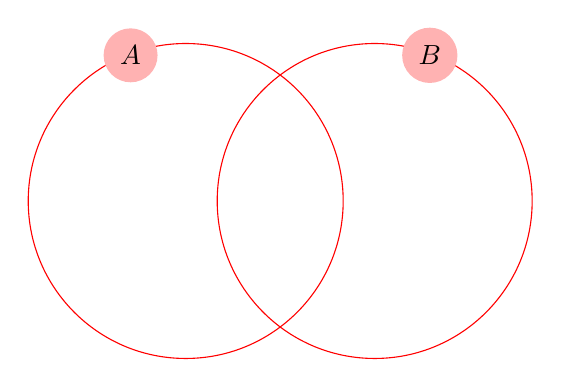
\begin{tikzpicture}

      \draw[red, thin] (0,0) circle[radius=2] node[black,circle,fill=red!30] at (-0.7,1.85) {$A$};
      \draw[red, thin] (2.4,0) circle[radius=2] node[black,circle,fill=red!30] at (3.1,1.85) {$B$};
      
    \end{tikzpicture}
  \end{center}

\begin{solution}

  $A - B = \big\{@q2sAdB@\big\}$

  $B - A = \big\{@q2sBdA@\big\}$

  $A \cap B = \big\{@q2sAiB@\big\}$

  % \begin{center}
  %   \begin{tikzpicture}
  %
  %     \draw[red, thin] (0,0) circle[radius=2] node[black,circle,fill=red!30] at (-0.7,1.85) {$A$};
  %     \draw[red, thin] (2.4,0) circle[radius=2] node[black,circle,fill=red!30] at (3.1,1.85) {$B$};
  %
  %     \node[black,thin] at (-1.1,0) {$1$};
  %     \node[black,thin] at (-0.5,1) {$2$};
  %     \node[black,thin] at (-0.5,-1) {$10$};
  %
  %     \node[black,thin] at (1.2,0.7) {$6$};
  %     \node[black,thin] at (1.2,0) {$8$};
  %     \node[black,thin] at (1.2,-0.7) {$16$};
  %     
  %     \node[black,thin] at (3.3,0) {$4$};
  %     \node[black,thin] at (2.7,1) {$12$};
  %     \node[black,thin] at (2.7,-1) {$14$};
  %
  %   \end{tikzpicture}
  % \end{center}
\end{solution}

\question[1]

Represente, na reta real, os intervalos:

\begin{tasks}
  \task $A = \big@q3A@\big@q3A2@$
  \task $B = \big\{x \in \mathbb{R} \,/\, @q3B@\big\}$
  \task $C = \big]-\infty, @q3C@\big@q3C2@$
  \task $D = \big\{x \in \mathbb{R} \,/\, @q3D@\big\}$
\end{tasks}

\begin{solution}[1in]

  % \begin{tasks}
  %   \task {
  %     \begin{tikzpicture}
  %       \tikzstyle{aberto}=[fill=white, draw=black, circle, inner sep=1.5pt]
  %       \tikzstyle{fechado}=[fill=black, draw=black, circle, inner sep=1.5pt]
  %
  %       \coordinate (A) at (-5,0);
  %       \coordinate (B) at (10,0);
  %       \coordinate (C) at (2,0);
  %       \coordinate (D) at (8,0);
  %
  %       \draw[thick, <->] (A) -- (B);
  %       \draw[red, ultra thick] (C) -- (D);
  %
  %       \node at (B)[below]{$\mathbb{R}$};
  %
  %       \node at (C)[fechado]{};
  %       \node at (C)[below]{$2$};
  %
  %       \node at (D)[fechado]{};
  %       \node at (D)[below]{$8$};
  %     \end{tikzpicture}
  %   }
  %   \task {
  %     \begin{tikzpicture}
  %       \tikzstyle{aberto}=[fill=white, draw=black, circle, inner sep=1.5pt]
  %       \tikzstyle{fechado}=[fill=black, draw=black, circle, inner sep=1.5pt]
  %
  %       \coordinate (A) at (-5,0);
  %       \coordinate (B) at (10,0);
  %       \coordinate (C) at (2,0);
  %       \coordinate (D) at (5,0);
  %
  %       \draw[thick, <->] (A) -- (B);
  %       \draw[red, ultra thick] (C) -- (D);
  %
  %       \node at (B)[below]{$\mathbb{R}$};
  %
  %       \node at (C)[aberto]{};
  %       \node at (C)[below]{$2$};
  %
  %       \node at (D)[aberto]{};
  %       \node at (D)[below]{$5$};
  %     \end{tikzpicture}
  %   }
  %   \task {
  %     \begin{tikzpicture}
  %       \tikzstyle{aberto}=[fill=white, draw=black, circle, inner sep=1.5pt]
  %       \tikzstyle{fechado}=[fill=black, draw=black, circle, inner sep=1.5pt]
  %
  %       \coordinate (A) at (-5,0);
  %       \coordinate (B) at (10,0);
  %       \coordinate (C) at (2,0);
  %
  %       \draw[thick, <->] (A) -- (B);
  %       \draw[red, ultra thick] (A) -- (C);
  %
  %       \node at (B)[below]{$\mathbb{R}$};
  %
  %       \node at (C)[fechado]{};
  %       \node at (C)[below]{$2$};
  %
  %     \end{tikzpicture}
  %   }
  %   \task {
  %     \begin{tikzpicture}
  %       \tikzstyle{aberto}=[fill=white, draw=black, circle, inner sep=1.5pt]
  %       \tikzstyle{fechado}=[fill=black, draw=black, circle, inner sep=1.5pt]
  %
  %       \coordinate (A) at (-5,0);
  %       \coordinate (B) at (10,0);
  %       \coordinate (C) at (-2,0);
  %       \coordinate (D) at (2,0);
  %
  %       \draw[thick, <->] (A) -- (B);
  %       \draw[red, ultra thick] (C) -- (D);
  %
  %       \node at (B)[below]{$\mathbb{R}$};
  %
  %
  %       \node at (C)[fechado]{};
  %       \node at (C)[below]{$-2$};
  %
  %       \node at (D)[fechado]{};
  %       \node at (D)[below]{$2$};
  %     \end{tikzpicture}
  %   }
  % \end{tasks}

\end{solution}

\question[2]

Uma editora estuda a possibilidade de lançar novamente as publicações: \textit{Helena}, \textit{Senhora} e \textit{A Moreninha}. 
Para isto, efetuou uma pesquisa de mercado e concluiu que em cada @q4t@ pessoas consultas:

\begin{itemize}
  \item @q4m@ leram \textit{A Moreninha};
  \item @q4h@ leram \textit{Helena};
  \item @q4s@ leram \textit{Senhora};
  \item @q4mh@ leram \textit{A Moreninha} e \textit{Helena};
  \item @q4ms@ leram \textit{A Moreninha} e \textit{Senhora};
  \item @q4sh@ leram \textit{Senhora} e \textit{Helena};
  \item @q4mhs@ leram as três obras.
\end{itemize}

Calcule:

\begin{tasks}
  \task O número de pessoas que leu apenas uma das obras.
  \task O número de pessoas que não leu nenhuma das obras.
  \task O número de pessoas que leu duas ou mais obras.
\end{tasks}

\begin{solution}[1in]
  \begin{center}
    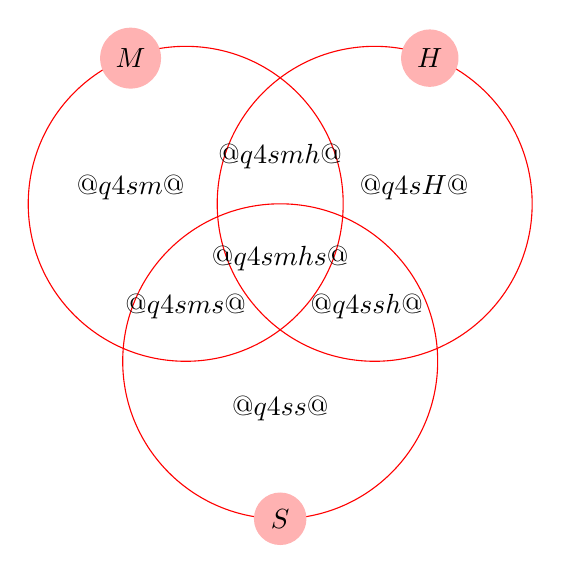
\begin{tikzpicture}

      \draw[red, thin] (0,0) circle[radius=2] node[black,circle,fill=red!30] at (-0.7,1.85) {$M$};
      \draw[red, thin] (2.4,0) circle[radius=2] node[black,circle,fill=red!30] at (3.1,1.85) {$H$};
      \draw[red, thin] (1.2,-2) circle[radius=2] node[black,circle,fill=red!30] at (1.2,-4) {$S$};

      \node[black,thin] at (-0.7,0.2) {$@q4sm@$};
      \node[black,thin] at (1.2,0.6) {$@q4smh@$};
      \node[black,thin] at (1.2,-0.7) {$@q4smhs@$};
      \node[black,thin] at (0,-1.3) {$@q4sms@$};
      \node[black,thin] at (2.3,-1.3) {$@q4ssh@$};
      \node[black,thin] at (2.9,0.2) {$@q4sH@$};
      \node[black,thin] at (1.2,-2.6) {$@q4ss@$};

    \end{tikzpicture}
  \end{center}
  
  \begin{tasks}
    \task $@q4sa@$
    \task $@q4sb@$
    \task $@q4sc@$
  \end{tasks}
  
\end{solution}

\question[2]

Em uma aula de Matemática, o professor propôs 2 problemas para serem resolvidos pela turma. 
$@q5AdB@\%$ dos alunos resolveram o primeiro problema. $@q5BdA@\%$ resolveram o segundo e $@q5nAuB@\%$ dos alunos 
não conseguiram resolver nenhum dos dois. Se apenas @q5nAiB@ alunos resolveram os dois problemas, pode-se 
concluir que o número de alunos dessa classe é:

\begin{tasks}(5)
  \task 100
  \task 150
  \task 200
  \task 250
  \task 300
\end{tasks}

\begin{solution}[2in]
  \begin{center}
    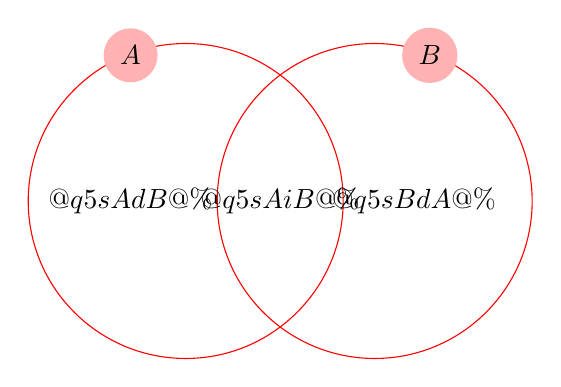
\begin{tikzpicture}

      \draw[red, thin] (0,0) circle[radius=2] node[black,circle,fill=red!30] at (-0.7,1.85) {$A$};
      \draw[red, thin] (2.4,0) circle[radius=2] node[black,circle,fill=red!30] at (3.1,1.85) {$B$};

      \node[black,thin] at (-0.7,0) {$@q5sAdB@\%$};
      \node[black,thin] at (1.2,0) {$@q5sAiB@\%$};
      \node[black,thin] at (2.9,0) {$@q5sBdA@\%$};

    \end{tikzpicture}
  \end{center}


  $200$

\end{solution}

\end{questions}
\end{document}
